\chapter{Docker Load Balancing with Nginx \\
\small{\textit{-- JG, CS}}}
\index{Docker}
\index{Nginx}
\index{Load Balancing}
\index{Chapter!Docker Load Balancing with Nginx}
\label{Chapter::LoadBalancing}

This project demonstrates a containerized load balancing setup using Docker and Nginx. The goal was to distribute incoming requests across multiple backend web servers to ensure reliability and scalability.

\section*{Environment Setup}
The environment consists of three Nginx containers: two backend servers (\texttt{web1} and \texttt{web2}) and one load balancer. Each backend container serves a unique static page to verify traffic distribution.

The containers were defined in a \texttt{docker-compose.yml} file, specifying the services, their networks, and volume mounts for the HTML content:

\begin{lstlisting}[language=yaml, caption={docker-compose.yml file}]
services:
  web1:
    image: nginx
    volumes:
      - ./web1:/usr/share/nginx/html
    networks:
      - lbnet

  web2:
    image: nginx
    volumes:
      - ./web2:/usr/share/nginx/html
    networks:
      - lbnet

  loadbalancer:
    image: nginx
    ports:
      - "8080:80"
    volumes:
      - ./nginx/nginx.conf:/etc/nginx/nginx.conf:ro
    depends_on:
      - web1
      - web2
    networks:
      - lbnet

networks:
  lbnet:
\end{lstlisting}

\section*{Load Balancer Configuration}
The load balancer uses Nginx's \texttt{upstream} directive to define the backend servers and distributes requests in a round-robin fashion. The configuration also forwards the original request headers to preserve client information:

\begin{lstlisting}[language=nginx, caption={nginx.conf for the load balancer}]
events {}

http {
    upstream backend {
        server web1:80;
        server web2:80;
    }

    server {
        listen 80;

        location / {
            proxy_pass http://backend;
            proxy_set_header Host $host;
            proxy_set_header X-Real-IP $remote_addr;
        }
    }
}
\end{lstlisting}

\section*{Testing and Verification}
After bringing up the containers using \texttt{docker compose up --build -d}, the backend servers responded with distinct pages. \texttt{web1} displayed:

\begin{figure}[h!]
    \centering
    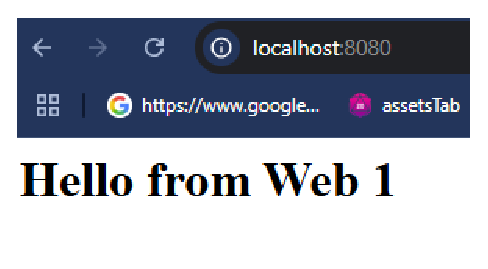
\includegraphics[width=0.7\linewidth]{eps/HelloFromWeb1.eps}
    \caption{Response from \texttt{web1} container}
\end{figure}

\noindent while \texttt{web2} displayed:

\begin{figure}[h!]
    \centering
    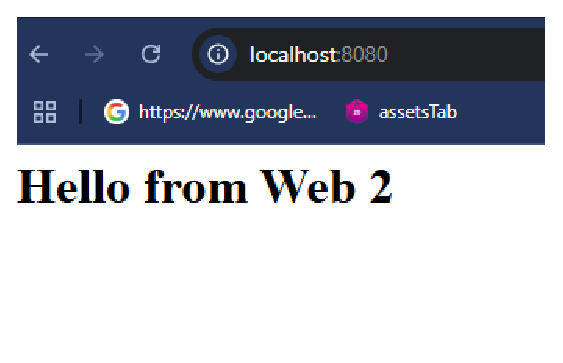
\includegraphics[width=0.7\linewidth]{eps/HelloFromWeb2.eps}
    \caption{Response from \texttt{web2} container}
\end{figure}

Repeatedly accessing the load balancer endpoint confirmed that requests were alternated between the two backend servers, demonstrating successful round-robin load balancing. The overall setup can be visualized as follows:

\begin{figure}[h!]
    \centering
    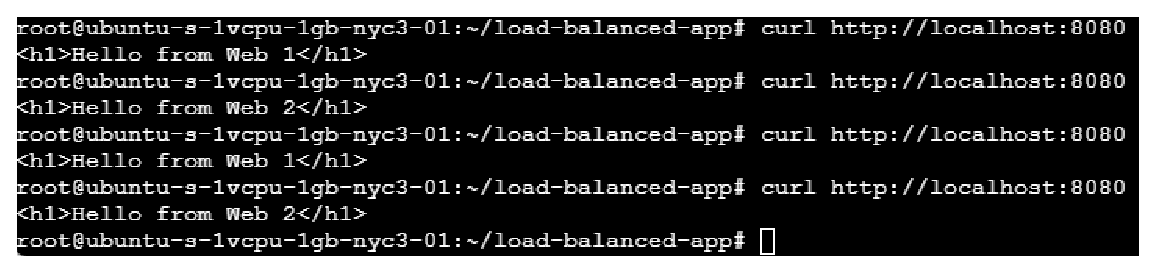
\includegraphics[width=0.9\linewidth]{eps/LoadBalancedApp.eps}
    \caption{Docker network showing load balancer distributing requests to backend servers}
\end{figure}

\section*{Conclusion}
The link to the load-balancer is here, at \url{http://157.245.10.33:8080/}

This project shows how Docker and Nginx can be combined to implement a simple load-balanced web service. The configuration ensures that multiple backend containers can serve traffic reliably and that scaling up is straightforward. By examining the responses from each container and observing alternating content at the load balancer endpoint, we verified that traffic distribution is working as expected.

